\chapter{Attachments}

\section{Source codes}
\label{sec:source_codes}

Source codes of PrankWeb are attached to this thesis in the ZIP archive. The archive contains all of the source codes, not only the work done in this thesis as the work was done in a fork of the same repository as the rest of the PrankWeb application. The directories that were added or intensively modified in this thesis are listed below:
\begin{itemize}
    \item \texttt{frontend} - contains the source codes of the frontend application
    \item \texttt{executor-docking} - contains the source codes of the docking plug-in
    \item \texttt{web-server} - contains the source codes of the Flask application
\end{itemize}

For the individual changed files, check the GitHub commits. For the current state of the source codes, check the GitHub repository.

\section{GitHub}
\label{sec:github}

The source codes are publicly available on GitHub at \url{https://github.com/cusbg/prankweb}.

The official documentation of the PrankWeb architecture and P2Rank tool is available at \url{https://github.com/cusbg/p2rank-framework/}.

The development was done in a fork of the PrankWeb repository at \url{https://github.com/luk27official/prankweb}.

\pagebreak
\section{Abbreviations}
\label{sec:abbreviations}
\begin{itemize}
    \item \textbf{1D} - one dimensional
    \item \textbf{3D} - three dimensional
    \item \textbf{ADFR} - AutoDockFR
    \item \textbf{API} - Application Programming Interface
    \item \textbf{CIF / mmCIF} - Macromolecular Crystallographic Information File
    \item \textbf{CSS} - Cascading Style Sheets
    \item \textbf{CSV} - Comma Separated Values
    \item \textbf{FASTA} - FAST-All
    \item \textbf{JRE} - Java Runtime Environment
    \item \textbf{JSX} - JavaScript Syntax Extension
    \item \textbf{JSON} - JavaScript Object Notation
    \item \textbf{PDB} - Protein Data Bank
    \item \textbf{PDBx} - Protein Data Bank eXtended
    \item \textbf{pLDDT} - per-residue Local Distance Difference Test
    \item \textbf{RCSB} - Research Collaboratory for Structural Bioinformatics
    \item \textbf{REST} - Representational State Transfer
    \item \textbf{SCSS} - Sassy CSS
    \item \textbf{SMILES} - Simplified Molecular Input Line Entry System
    \item \textbf{WSGI} - Web Server Gateway Interface
\end{itemize}


\section{Pocket detail designs}
\label{sec:pocket_detail_designs}

This section contains all pocket detail designs that were considered for displaying more information about a pocket. In the end, the \cref{fig:dialog-4} was chosen. For more information refer to \cref{sec:plugins}.

\begin{figure}[htb]
    \centering
    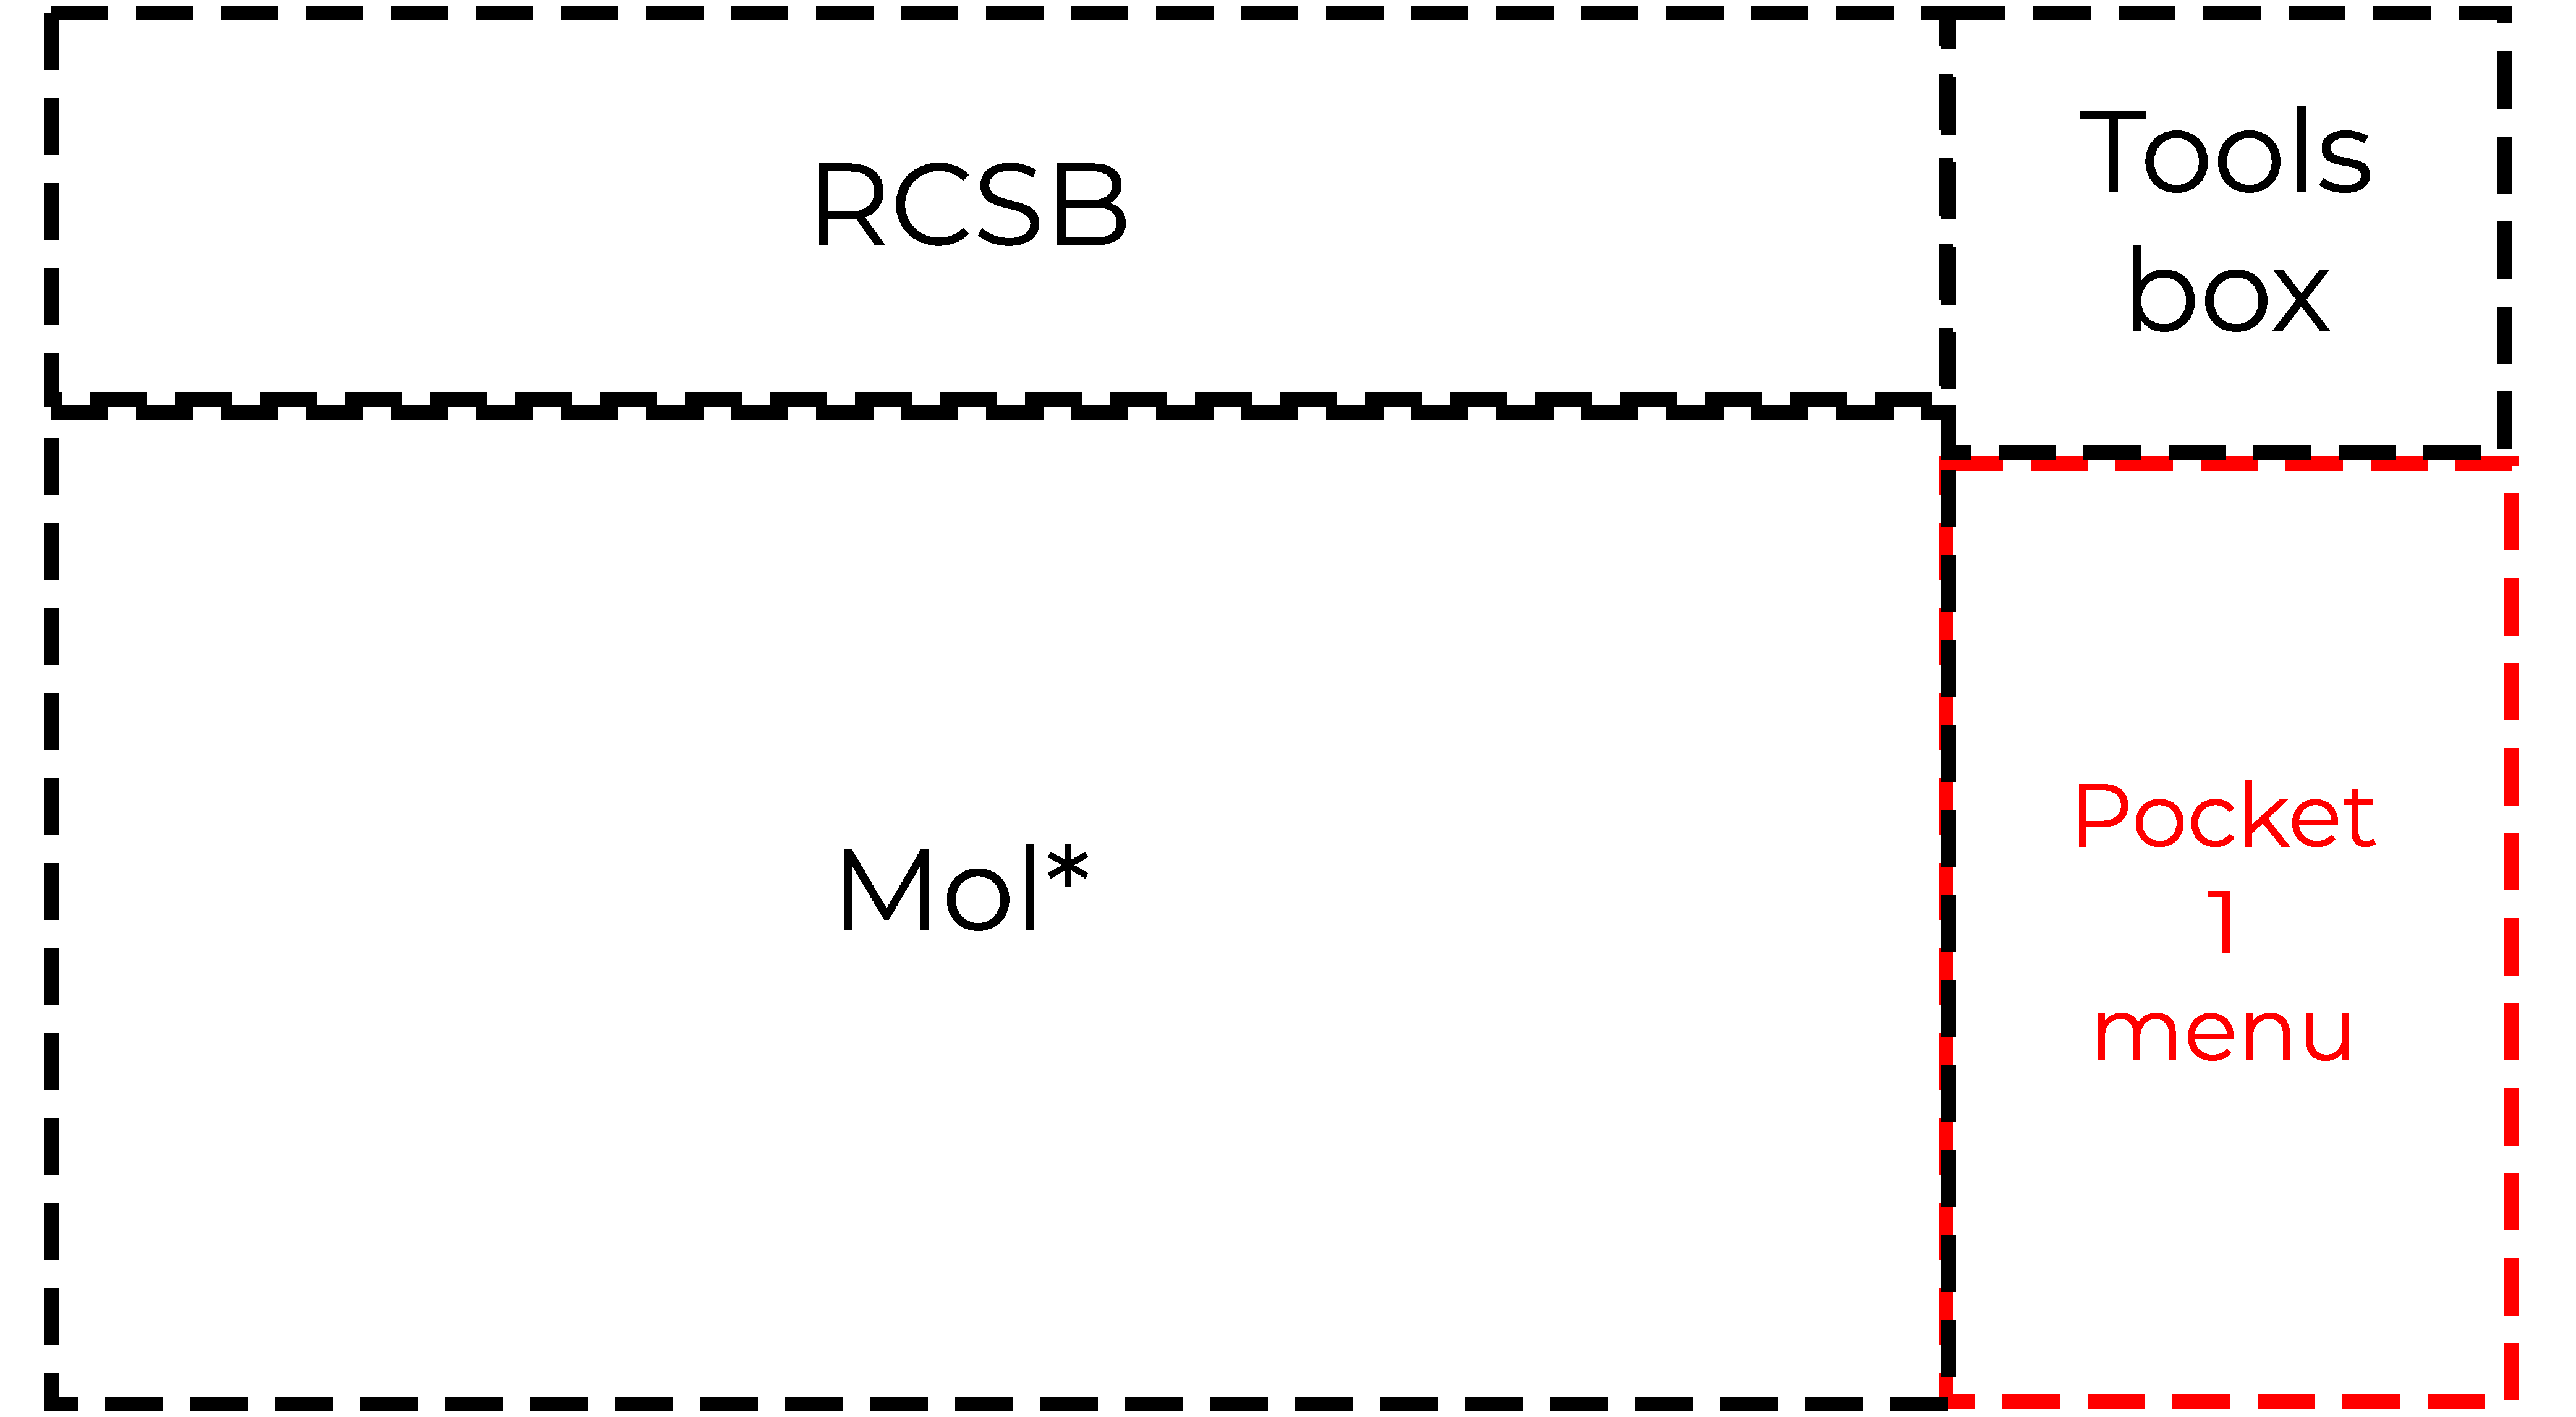
\includegraphics[width=1\linewidth]{img/dialog_1-svg.pdf}
    \caption{The first option for displaying pocket information.}
    \label{fig:figure-1}
\end{figure}

\begin{figure}[htb]
    \centering
    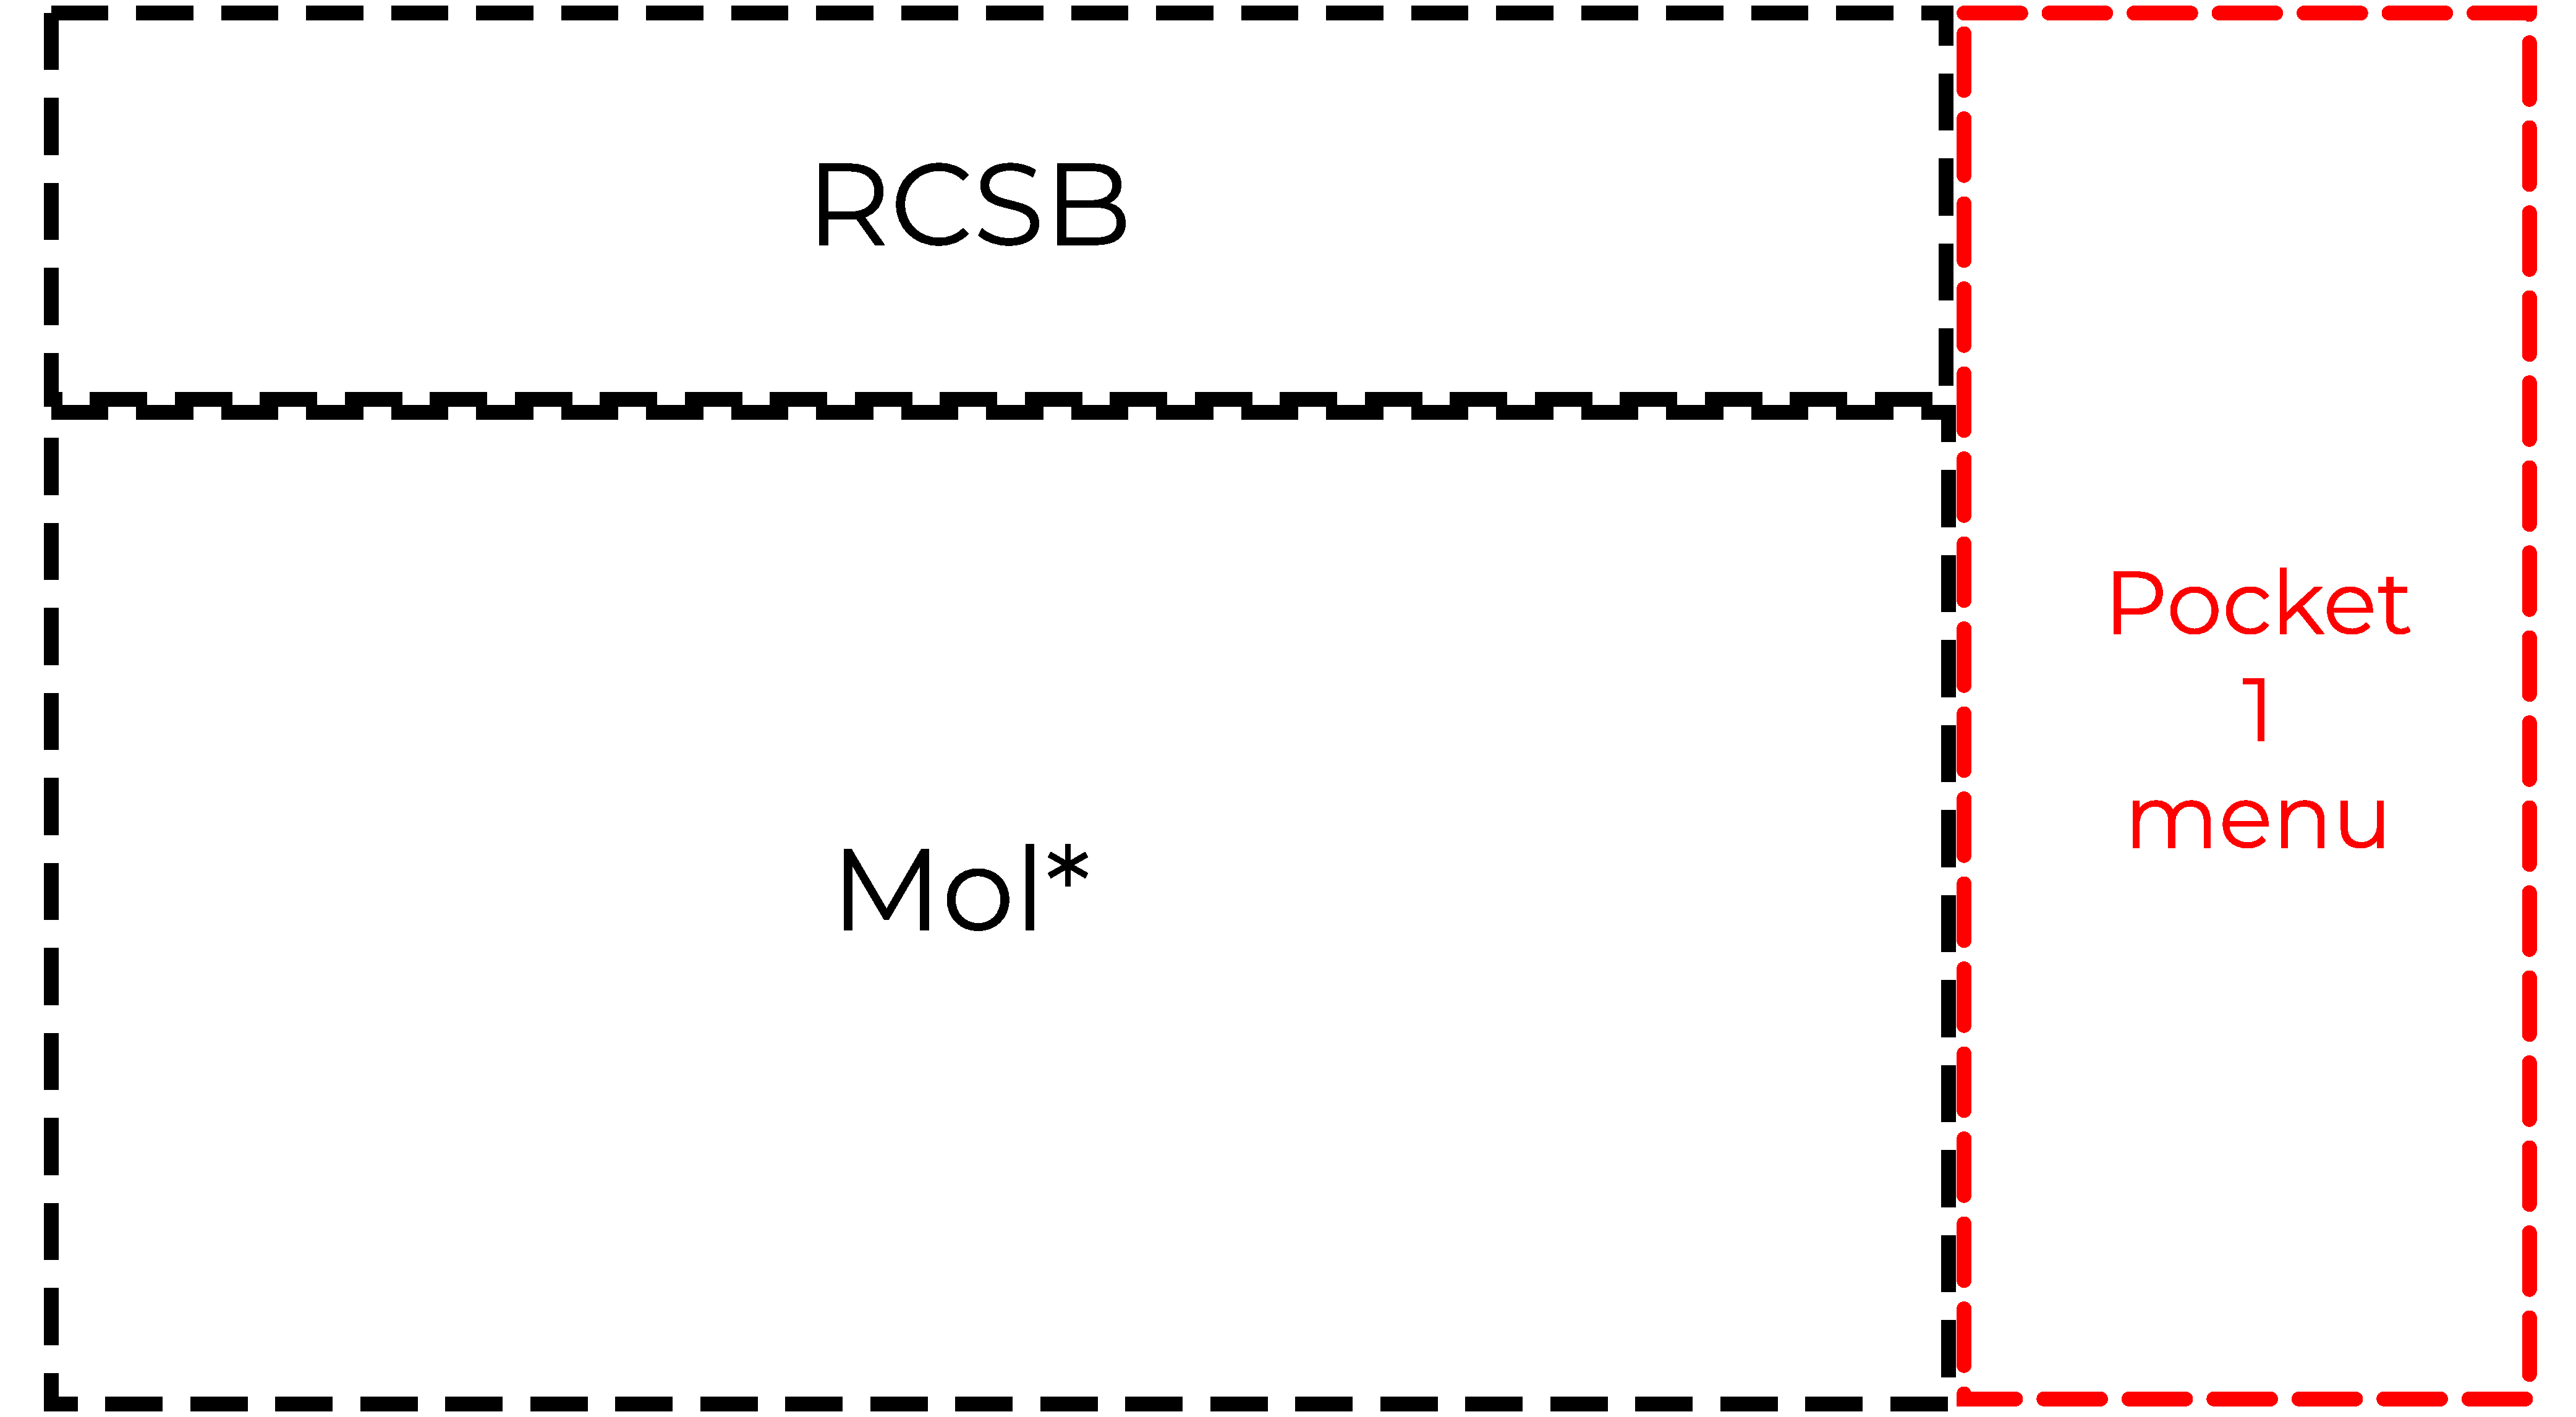
\includegraphics[width=1\linewidth]{img/dialog_2-svg.pdf}
    \caption{The second option for displaying pocket information.}
    \label{fig:figure-2}
\end{figure}

\begin{figure}[htb]
	\centering
	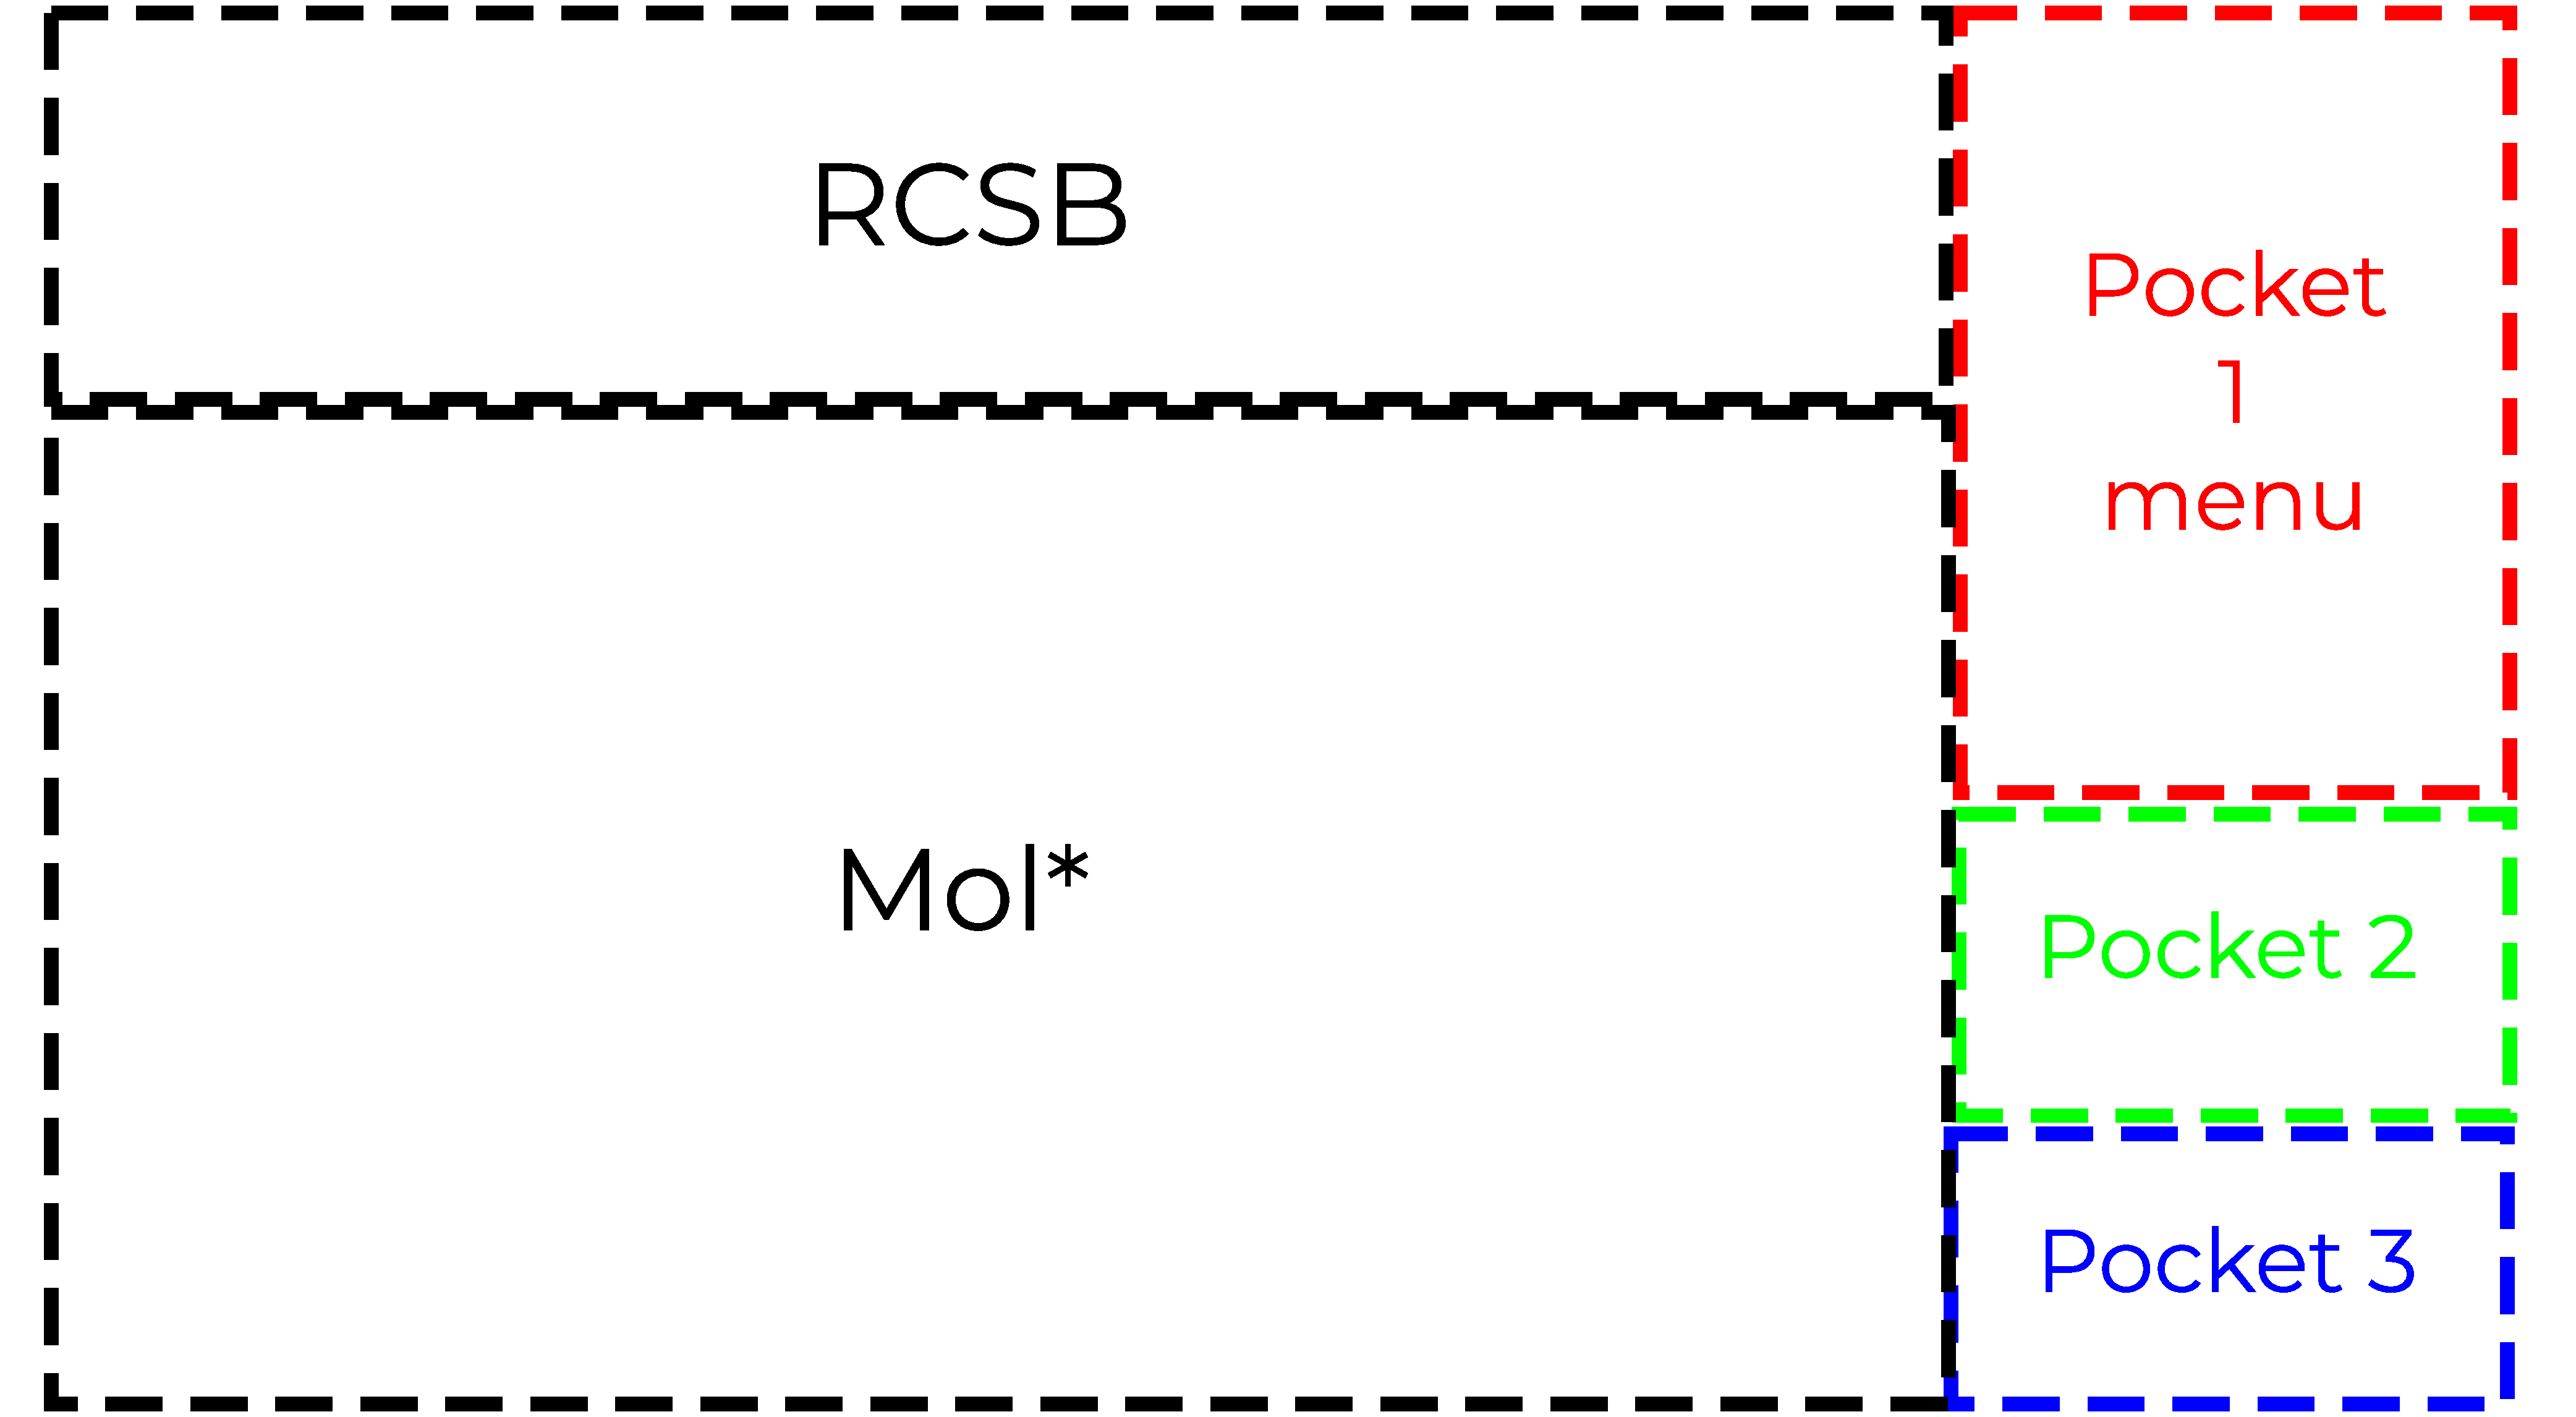
\includegraphics[width=1\linewidth]{img/dialog_3-svg.pdf}
	\caption{The third option for displaying pocket information.}
	\label{fig:figure-3}
\end{figure}

\begin{figure}[htb]
	\centering
	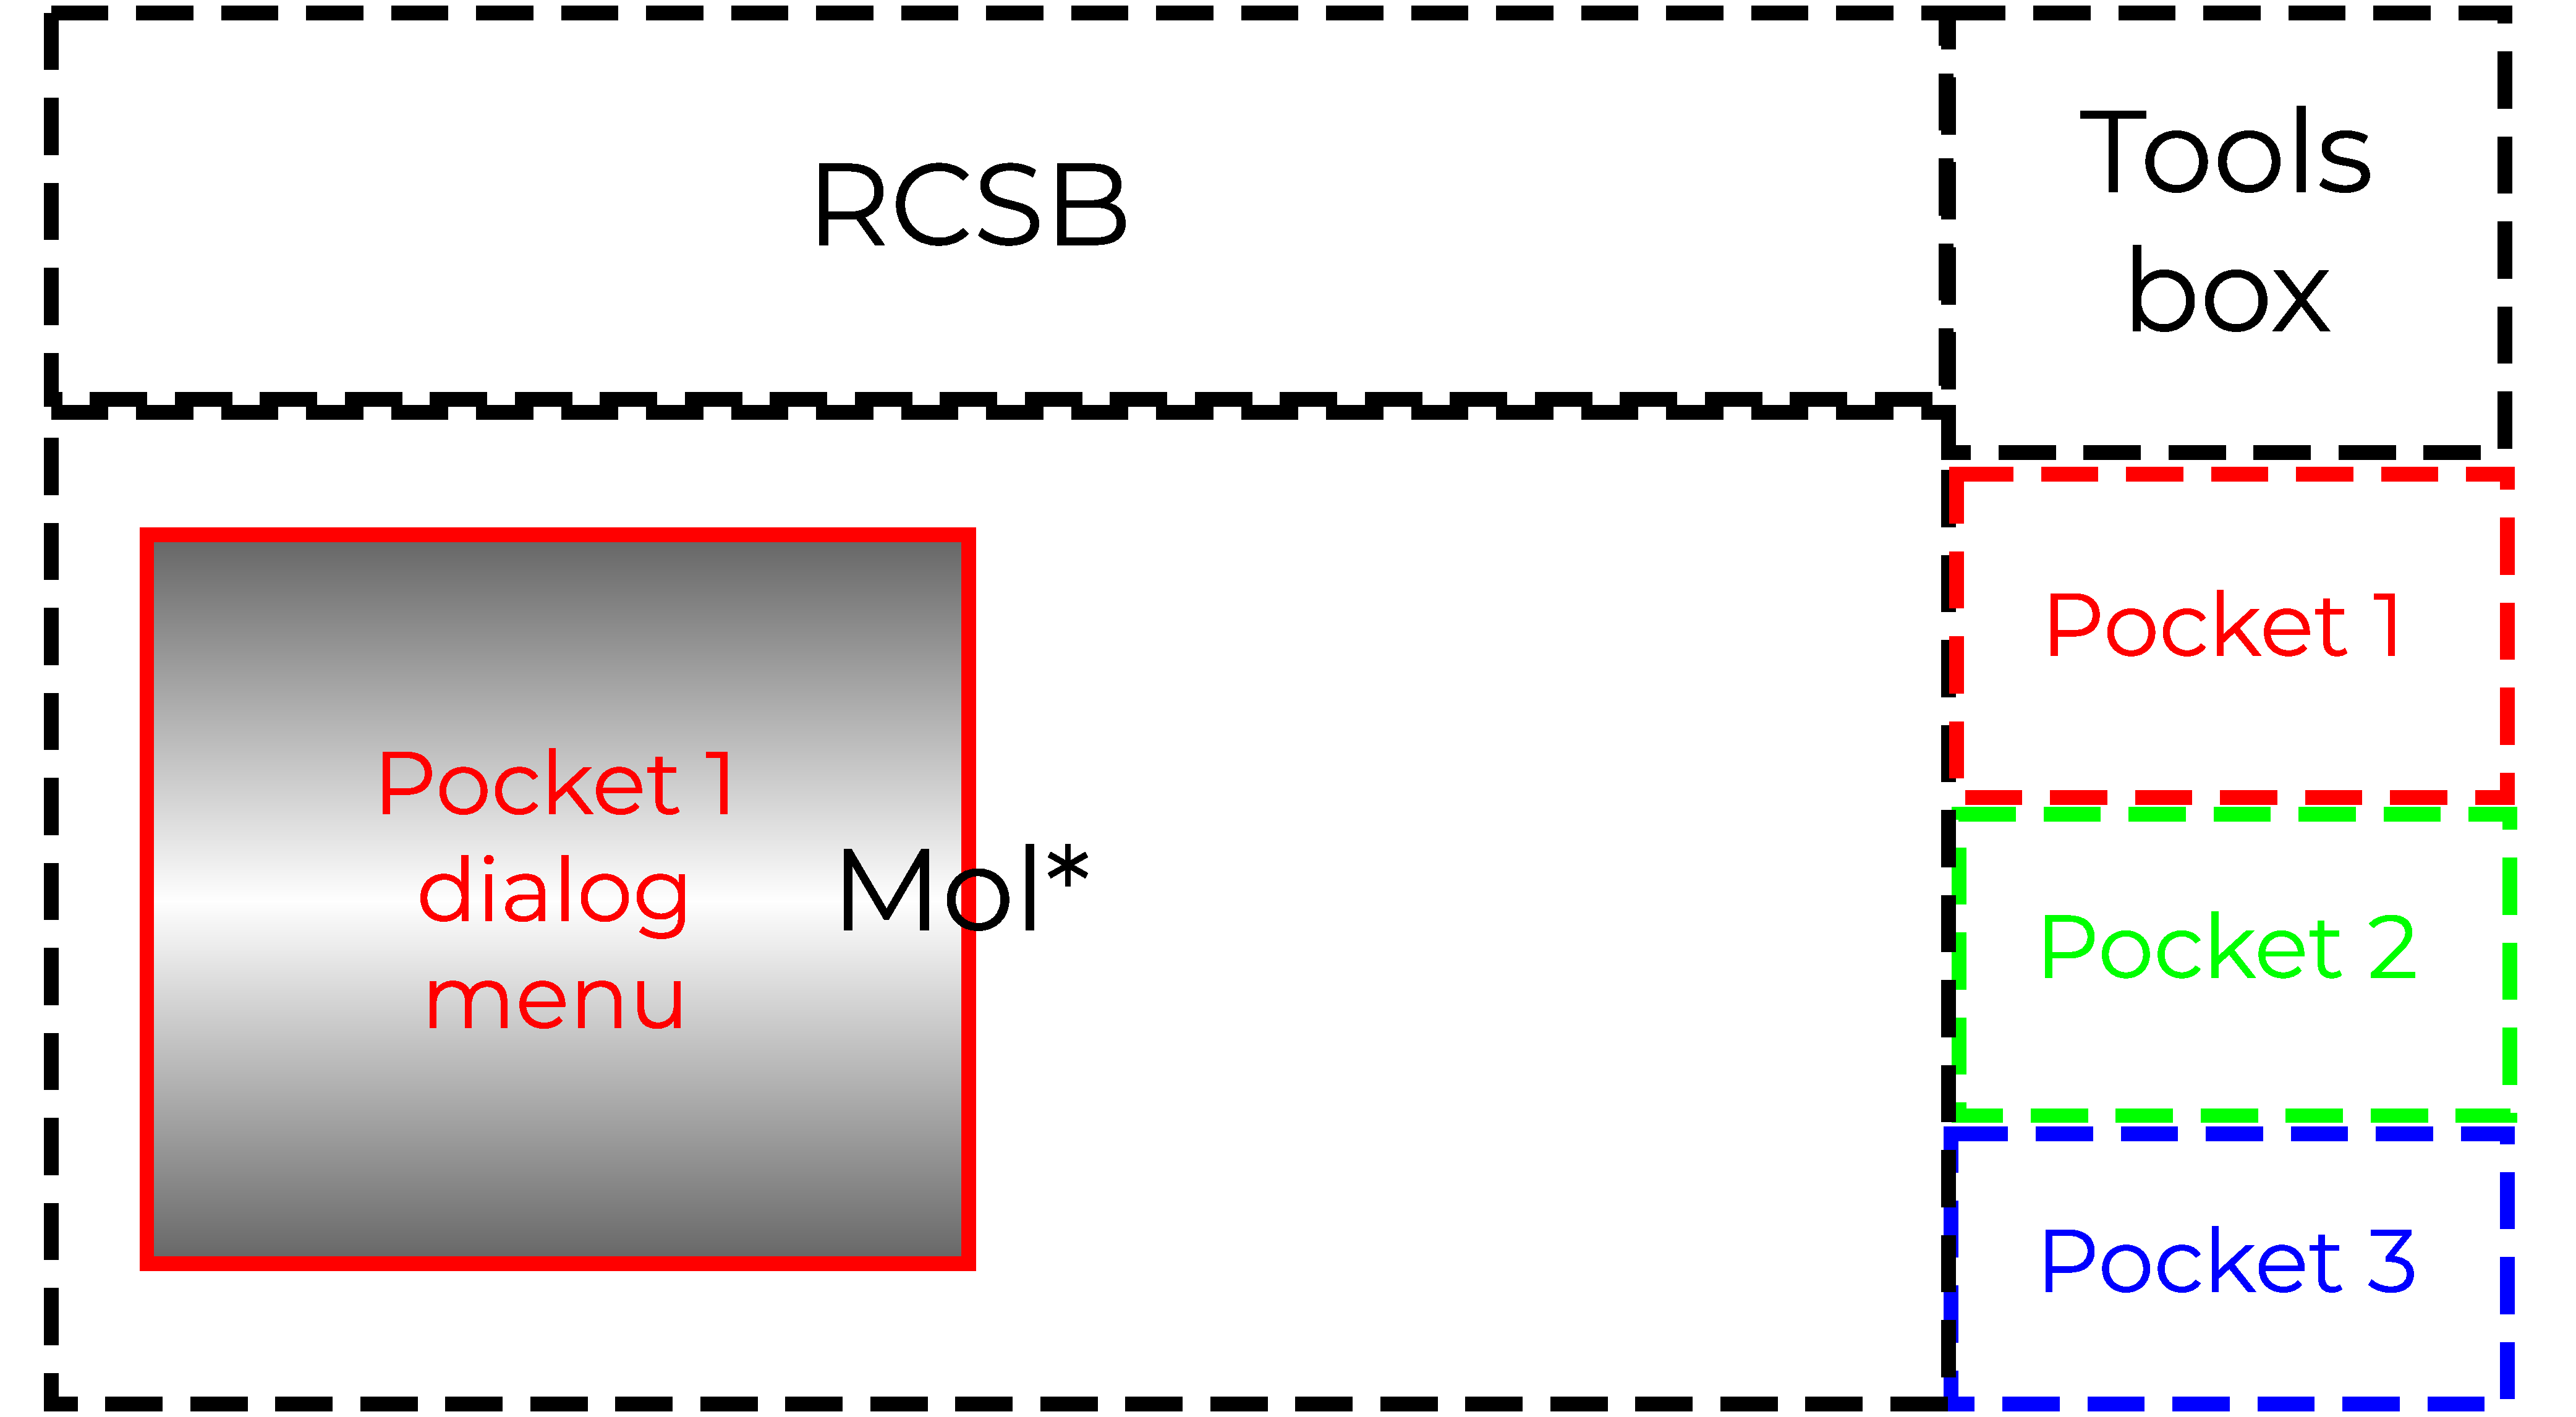
\includegraphics[width=1\linewidth]{img/dialog_4-svg.pdf}
	\caption{The fourth and chosen option for displaying pocket information.}
	\label{fig:dialog-4}
\end{figure}